\documentclass[border=15pt,tikz]{standalone}
\usepackage{amsmath}
\usetikzlibrary{arrows.meta, fit, positioning, backgrounds}
\usepackage[outline]{contour}
\contourlength{1.4pt}

\usepackage{helvet}
\renewcommand{\familydefault}{\sfdefault}
\usepackage{sansmath}
\sansmath

% --- COLOR DEFINITIONS (Okabe-Ito based: Graph construction=vermillion, GraphSAGE=navy, Hungarian=#2ecc71) ---
\usepackage{xcolor}
\definecolor{myred}{HTML}{e74c3c}
\definecolor{myblue}{HTML}{000080}
\definecolor{mygreen}{HTML}{D55E00}
\definecolor{myorange}{HTML}{E69F00}
\definecolor{myviolet}{HTML}{2ecc71}
\colorlet{mydarkred}{myred!30!black}
\colorlet{mydarkblue}{myblue!40!black}
\colorlet{mydarkgreen}{mygreen!30!black}
\colorlet{mydarkviolet}{myviolet!40!black}

% --- STYLES ---
\tikzset{
  >=latex,
  base node/.style={thick, circle, minimum size=22pt, inner sep=1pt, align=center, font=\scriptsize},
  node graph/.style={base node, draw=mygreen!40!black, fill=mygreen!15},
  op block/.style={thick, rounded corners=4pt, draw=myblue!40!black, fill=myblue!12, minimum width=3.6cm, minimum height=0.7cm, align=center, font=\small, inner sep=4pt},
  cell/.style={draw=mydarkviolet, thick, minimum width=0.85cm, minimum height=0.62cm, align=center, font=\scriptsize, fill=myviolet!6},
  cell win/.style={cell, fill=myviolet!30, draw=myviolet, ultra thick},
  inter edge/.style={thick, mygreen, shorten >=2pt, shorten <=2pt},
  intra edge/.style={thick, dashed, mydarkgreen!70!black, shorten >=2pt, shorten <=2pt},
  flow arrow/.style={->, thick, line width=1.5pt, draw=black!60},
  label/.style={font=\small\bfseries, align=center},
  desc/.style={font=\scriptsize, align=center, text=black!80},
  box/.style={draw, thick, rounded corners=6pt, inner sep=14pt, fill opacity=0.05}
}

\begin{document}

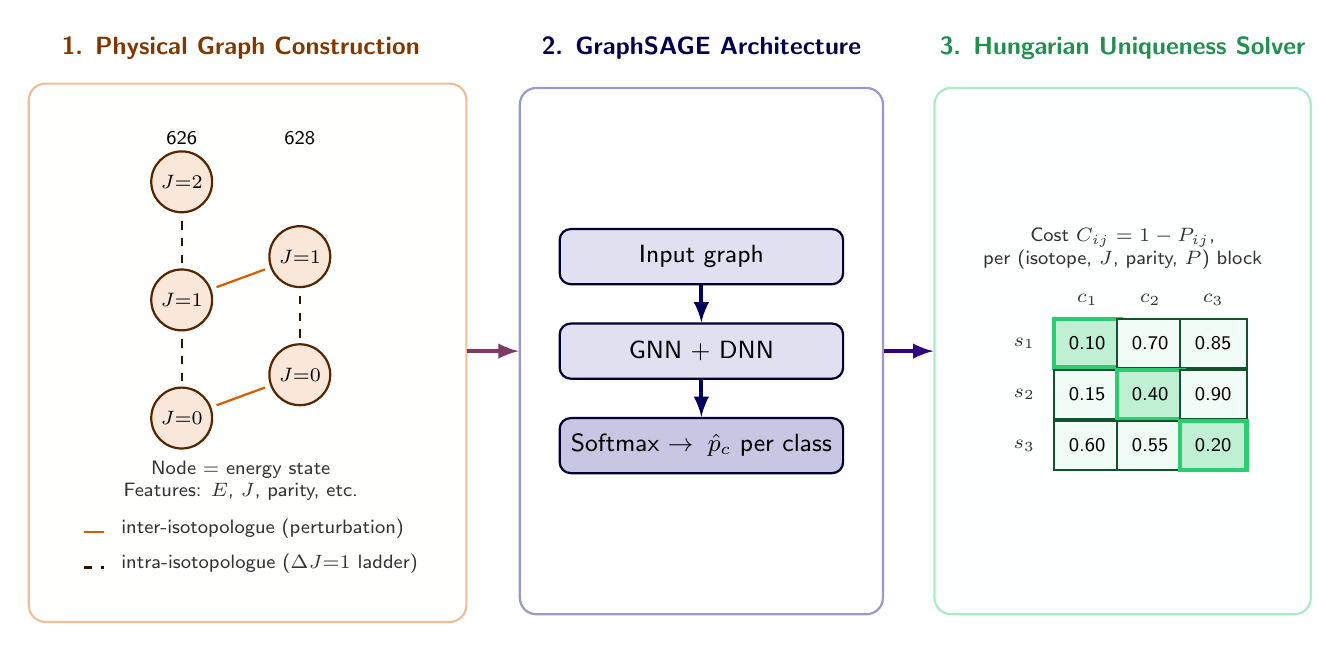
\begin{tikzpicture}[font=\sffamily]

  % =================================================================================
  % PANEL 1: PHYSICAL GRAPH CONSTRUCTION
  % =================================================================================

  \node[label, font=\scriptsize] (col626) at (0.0, 2.85) {626};
  \node[label, font=\scriptsize] (col628) at (1.5, 2.85) {628};

  \node[node graph] (A0) at (0.0, -0.7) {$J{=}0$};
  \node[node graph] (A1) at (0.0, 0.8) {$J{=}1$};
  \node[node graph] (A2) at (0.0, 2.3) {$J{=}2$};
  \node[node graph] (B0) at (1.5, -0.15) {$J{=}0$};
  \node[node graph] (B1) at (1.5, 1.35) {$J{=}1$};

  % Intra-isotopologue rotational ladder (Delta J = 1)
  \draw[intra edge] (A0) -- (A1);
  \draw[intra edge] (A1) -- (A2);
  \draw[intra edge] (B0) -- (B1);

  % Inter-isotopologue perturbation edges (shared polyad, J, parity)
  \draw[inter edge] (A0) -- (B0);
  \draw[inter edge] (A1) -- (B1);

  \node[label, mygreen!60!black] at (0.75, 4.0) (Title1) {1. Physical Graph Construction};

  % Subheading inside the panel, between the graph and the legend
  \node[desc] (p1desc) at (0.75, -1.5) {Node = energy state\\Features: $E$, $J$, parity, etc.};

  % Legend: explicit coordinates, one line per entry (no text width, no wrapping)
  \node[desc, anchor=west] (leg1a) at (-1.45, -2.1) {\tikz{\draw[inter edge] (0,0) -- (0.4,0);}\, inter-isotopologue (perturbation)};
  \node[desc, anchor=west] (leg1b) at (-1.45, -2.55) {\tikz{\draw[intra edge] (0,0) -- (0.4,0);}\, intra-isotopologue ($\Delta J{=}1$ ladder)};

  % Invisible corners give all three panels identical top/bottom edges
  \coordinate (p1t) at (0.75, 3.0);
  \coordinate (p1b) at (0.75, -2.7);
  \begin{pgfonlayer}{background}
    \node[box, fit=(col626) (col628) (A0) (A2) (B0) (B1) (p1desc) (leg1a) (leg1b) (p1t) (p1b), fill=mygreen!5, draw=mygreen!40] (panel1) {};
  \end{pgfonlayer}


  % =================================================================================
  % PANEL 2: GRAPHSAGE ARCHITECTURE (condensed)
  % =================================================================================

  \node[op block] (G1) at (6.6, 1.35)  {Input graph};
  \node[op block] (G2) at (6.6, 0.15)  {GNN + DNN};
  \node[op block, fill=myblue!22] (G3) at (6.6, -1.05) {Softmax $\rightarrow\; \hat p_c$ per class};

  \draw[flow arrow, draw=myblue!70!black] (G1) -- (G2);
  \draw[flow arrow, draw=myblue!70!black] (G2) -- (G3);

  \node[label, myblue!60!black] at (6.6, 4.0) (Title2) {2. GraphSAGE Architecture};

  \coordinate (p2t) at (6.6, 3.0);
  \coordinate (p2b) at (6.6, -2.7);
  \begin{pgfonlayer}{background}
    \node[box, fit=(G1) (G2) (G3) (p2t) (p2b), fill=myblue!5, draw=myblue!40] (panel2) {};
  \end{pgfonlayer}


  % =================================================================================
  % PANEL 3: HUNGARIAN UNIQUENESS SOLVER (cost matrix only)
  % =================================================================================

  \node[label, myviolet!70!black] at (11.95, 4.0) (Title3) {3. Hungarian Uniqueness Solver};

  \node[desc] (costlbl) at (11.95, 1.45) {Cost $C_{ij} = 1 - P_{ij}$,\\per (isotope, $J$, parity, $P$) block};

  % Column / row headers
  \node[desc] (c1h) at (11.5, 0.8) {$c_1$};
  \node[desc] (c2h) at (12.3, 0.8) {$c_2$};
  \node[desc] (c3h) at (13.1, 0.8) {$c_3$};
  \node[desc] (s1h) at (10.7, 0.25)  {$s_1$};
  \node[desc] (s2h) at (10.7, -0.4)  {$s_2$};
  \node[desc] (s3h) at (10.7, -1.05) {$s_3$};

  % Cost per (state, class) inside each square; bold cells = Hungarian assignment
  \node[cell win] (s1c1) at (11.5, 0.25)  {0.10};
  \node[cell]     (s1c2) at (12.3, 0.25)  {0.70};
  \node[cell]     (s1c3) at (13.1, 0.25)  {0.85};
  \node[cell]     (s2c1) at (11.5, -0.4)  {0.15};
  \node[cell win] (s2c2) at (12.3, -0.4)  {0.40};
  \node[cell]     (s2c3) at (13.1, -0.4)  {0.90};
  \node[cell]     (s3c1) at (11.5, -1.05) {0.60};
  \node[cell]     (s3c2) at (12.3, -1.05) {0.55};
  \node[cell win] (s3c3) at (13.1, -1.05) {0.20};

  \coordinate (p3t) at (11.95, 3.0);
  \coordinate (p3b) at (11.95, -2.7);
  \begin{pgfonlayer}{background}
    \node[box, fit=(costlbl) (c1h) (s1h) (s1c1) (s3c3) (p3t) (p3b), fill=myviolet!5, draw=myviolet!40] (panel3) {};
  \end{pgfonlayer}


  % =================================================================================
  % MACRO FLOW CONNECTIONS
  % =================================================================================

  % Horizontal arrows at a fixed height so panel-size differences don't slant them
  \draw[flow arrow, draw=mygreen!60!blue]   (panel1.east |- 0,0.15) -- (panel2.west |- 0,0.15);
  \draw[flow arrow, draw=myblue!60!violet]  (panel2.east |- 0,0.15) -- (panel3.west |- 0,0.15);

\end{tikzpicture}

\end{document}
